\section{Real-Time On-Board Deep Learning Fault Detection for Autonomous UAV
Inspections}

%1
\begin{frame}
    \frametitle{\textit{Real-Time On-Board Deep Learning Fault Detection for
    Autonomous UAV Inspections} ~------~ Overview}

    \begin{block}{The main task:}
        A UAV detection system based on the rotating wing drones and nvidia onboard
        computer is developed and implemented in this paper.
    \end{block}

    \begin{itemize}
        \item several object detection algorithms like SSD, YOLO, and RCNN are
            introduced in the beginning of this paper.
        \item the hardware platform are compared.
    \end{itemize}

    \begin{figure}[H]
        \centering
        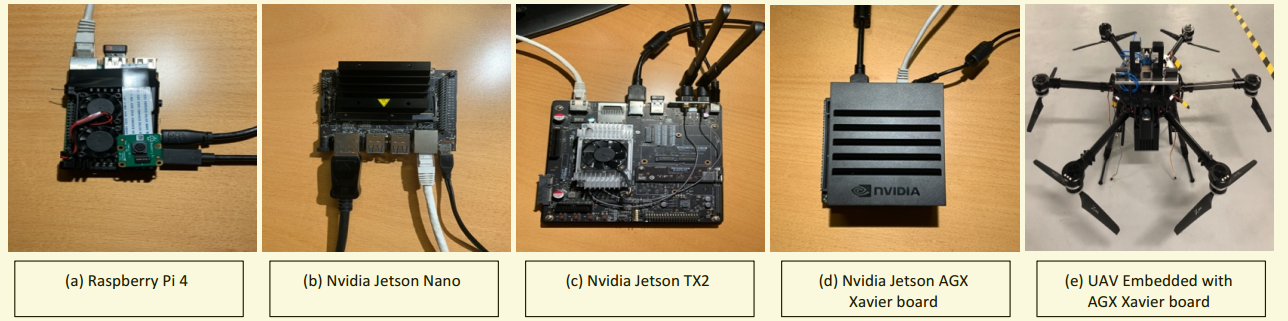
\includegraphics[width=0.9\textwidth]{./imgs/hardwares.png}
    \end{figure}

\end{frame}

%2
\begin{frame}
    \frametitle{\textit{Real-Time On-Board Deep Learning Fault Detection for
    Autonomous UAV Inspections} ~------~ Result}

    \begin{itemize}
        \item YOLO-v3, YOLO-v3-tiny, YOLO-v4, and YOLO-v4-tiny are developed and
            tested on the dataset.
        \item The YOLO-v4-tiny has the best performance.
    \end{itemize}

    \begin{figure}[H]
        \centering
        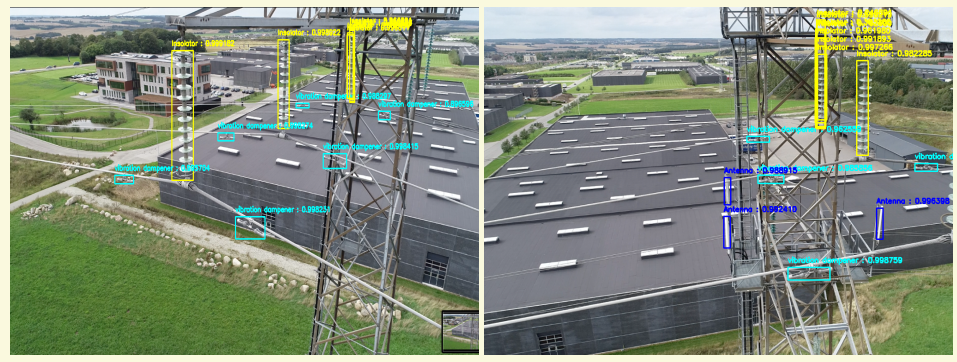
\includegraphics[width=0.9\textwidth]{./imgs/yolo_result.png}
    \end{figure}

\end{frame}
